\documentclass[12]{article}%12pt即为*四号字
\usepackage{ctex}%引入中文包
\usepackage{graphicx}%插入图片的包
\usepackage{geometry}%设置A4纸页边距的包
\usepackage{url}
\usepackage{stfloats}
\usepackage{float}

\geometry{left=3.18cm,right=3.18cm,top=2.54cm,bottom=2.54cm}%设置页边距
\linespread{1}%设置行间距



\begin{document}
\begin{center}
    \LARGE\songti\textbf{Chapter 2 Programming Assignments} \\%标题
    \large\kaishu\textbf{褚朱钇恒\qquad 3200104144}%一般是我的姓名
\end{center}
    \section{Programming Assignments}
        \subsection{A}
            在$NewtonInterpolation.h$中实现了牛顿插值类,提供了需要两个$vector$分别表示插值点$X$和点值$Y$的初始化函数$init$。同时为了发挥牛顿法的优越性,即在加入新插值点后只需要$\Theta(n)$的复杂度更新信息,还提供了$add\_node$接口以增加新插值点。

            为在$D$题中使用Hermite插值,该类还实现了$Hermite\_init\_and\_inter$函数,用于提供插值点$X$和插值点上的函数值与各阶导数值$Y$。

            输入所有插值点信息后,可以使用$()$进行求值,求值时将判断是否已计算出所有差商,如果没有将自动进行插值计算差商。
        
        \subsection{B}

            根据题意实现插值的效果如下:
            \begin{figure}[H]
                \centering
                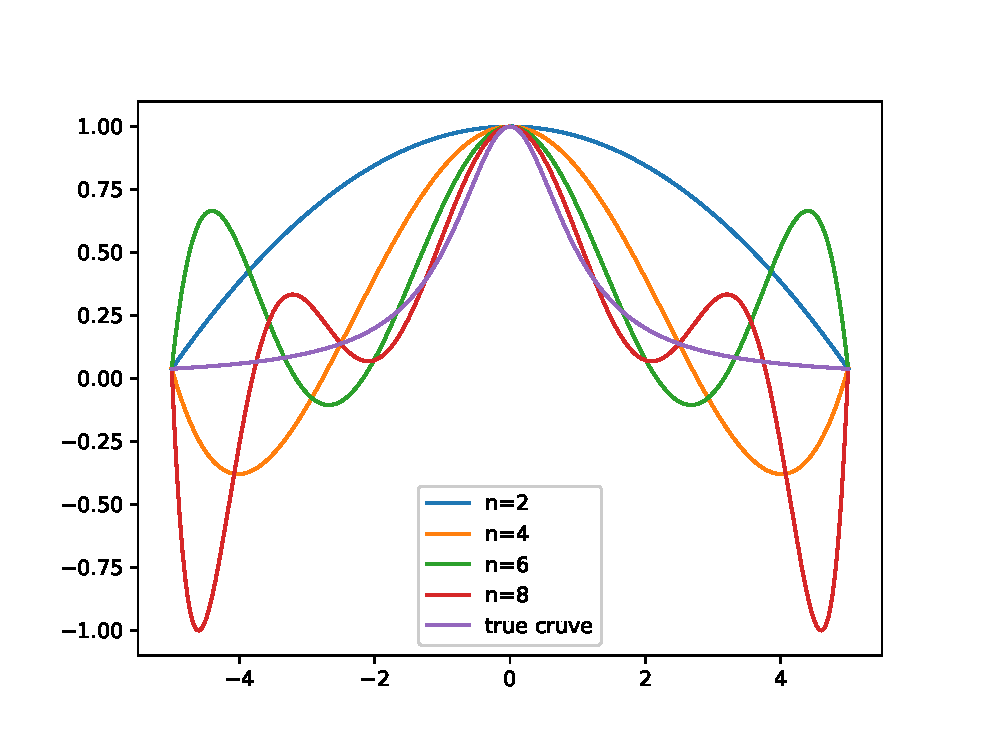
\includegraphics[width=0.7\textwidth]{./pic/B.eps}
                \caption{$f(x)=\frac{1}{1+x^2}$的插值结果}
            \end{figure}

            容易发现,在插值点序列的两端的震荡很大,出现了龙格现象。
        
        \subsection{C}
            使用$Chebyshev$插值点的插值结果如下:

            \begin{figure}[H]
                \centering
                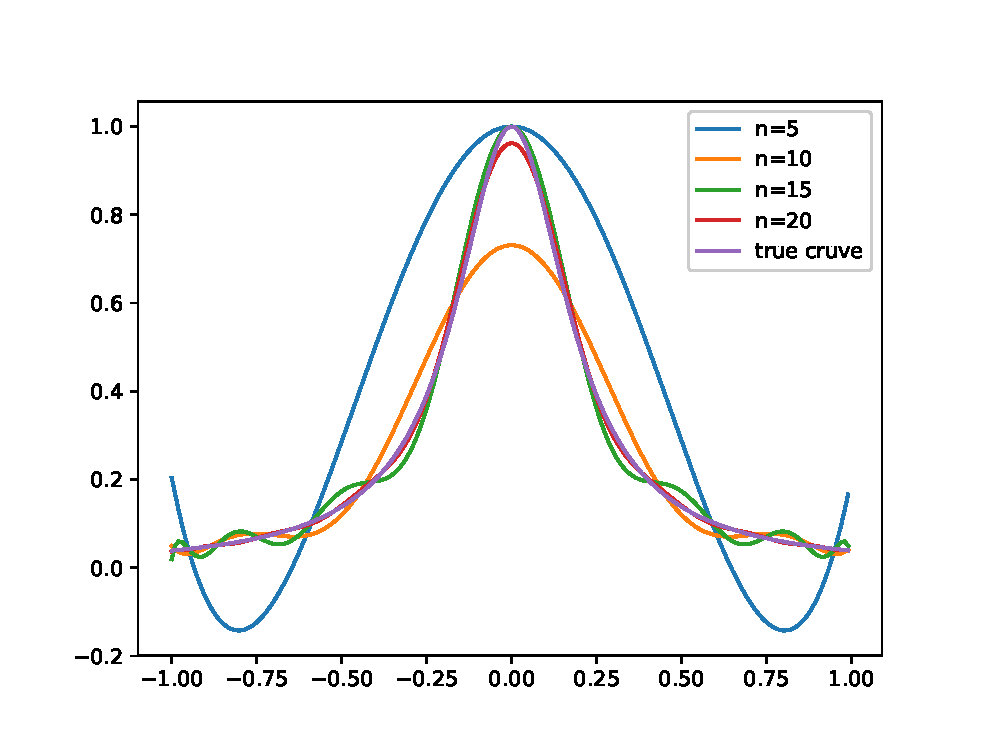
\includegraphics[width=0.7\textwidth]{./pic/C.eps}
                \caption{$f(x)=\frac{1}{1+25x^2}$的插值结果}
            \end{figure}

            容易发现,随着$n$的增大,插值点序列两端的震荡现象出现了很快的衰减,拟合效果较好。
        
        \subsection{D}
            \begin{figure}[H]
            \centering
            \begin{minipage}[t]{0.49\textwidth}
            \centering
            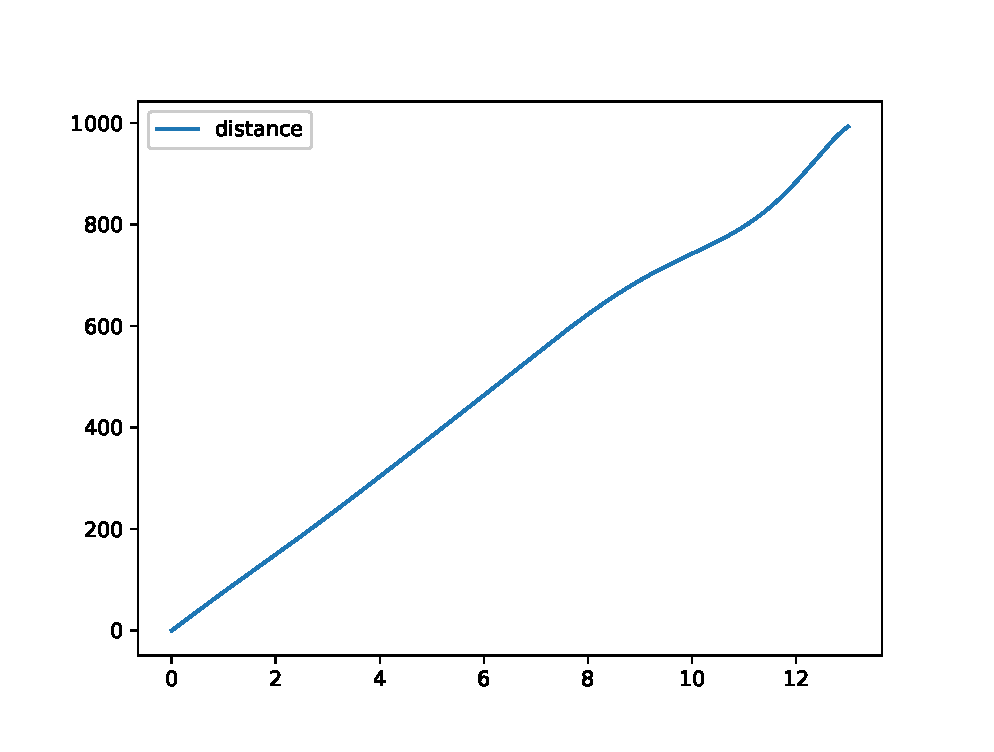
\includegraphics[width=7cm]{./pic/D_dis.eps}
            \caption{路程插值结果}
            \end{minipage}
            \begin{minipage}[t]{0.49\textwidth}
            \centering
            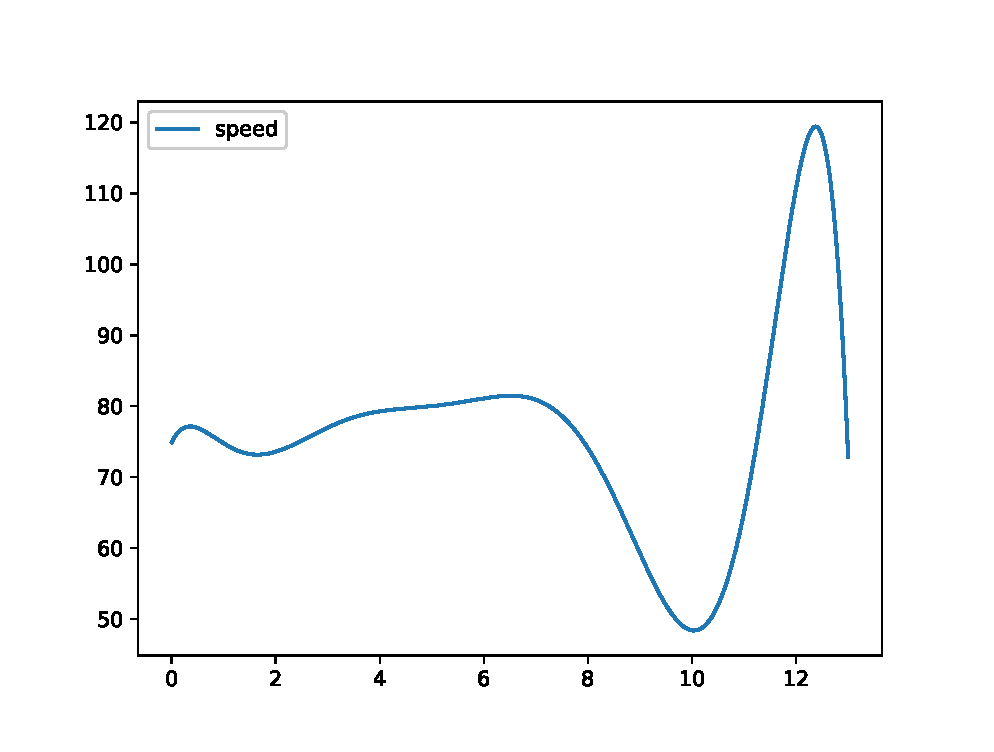
\includegraphics[width=7cm]{./pic/D_speed.eps}
            \caption{速度插值结果}
            \end{minipage}
            \end{figure}
            \subsubsection{a}
                使用Herimte插值得到$f(10)=742.503,f^{'}(10)=48.3822$,故$t=10s$时车的位置约为$742\ feet$,速度约为$48\ feet/s$。
            \subsubsection{b}
                根据速度插值结果图可以发现,车速最快约为$120\ feet/s$,超过了$81\ feet/s$的限速。
        
        \subsection{E}
            \subsection{a}
                使用牛顿插值法求得结果如下:
                \begin{figure}[H]
                    \centering
                    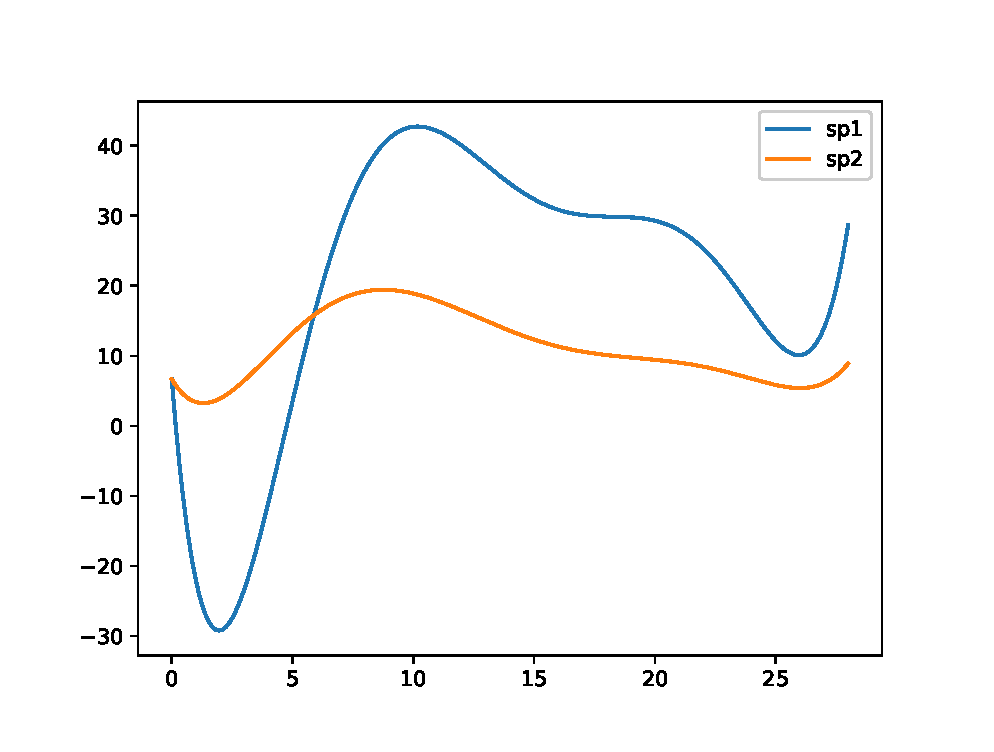
\includegraphics[width=0.7\textwidth]{./pic/E_1.eps}
                    \caption{Average weight curve}
                \end{figure}
            \subsubsection{b}
                发现之前求得的函数先出现了负值,然后再升高,显然不合理,故删除前几个采样点,重新拟合曲线预测未来趋势,结果如下:
                
                \begin{figure}[H]
                    \centering
                    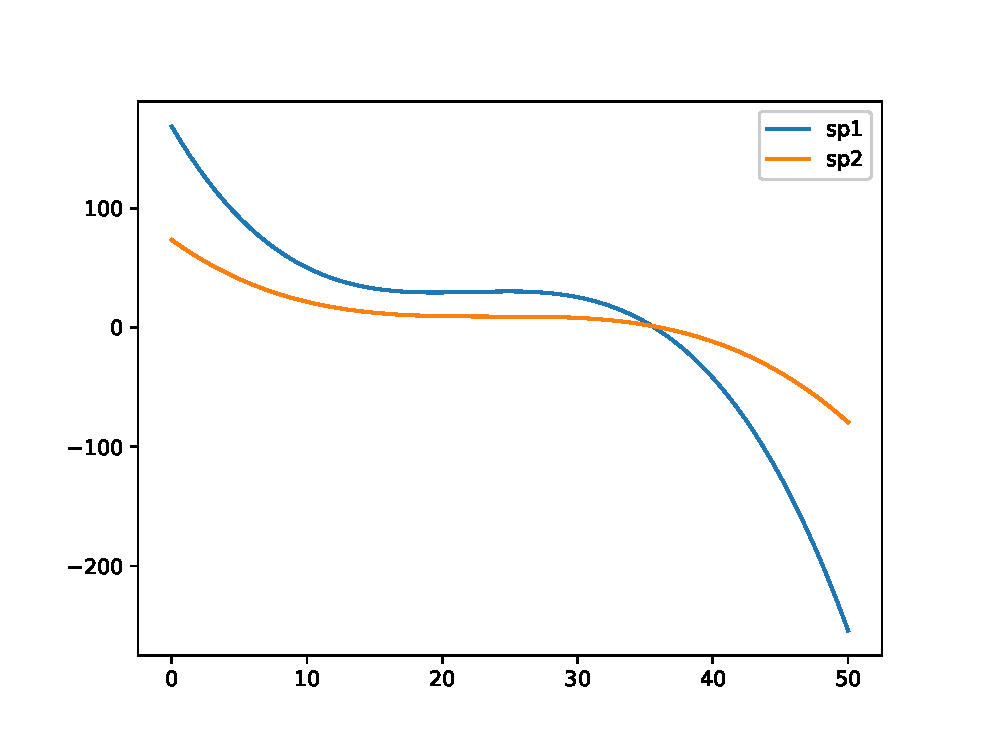
\includegraphics[width=0.7\textwidth]{./pic/E_2.eps}
                    \caption{Average weight curve}
                \end{figure}
                
                发现未来(约37d)函数值都将变负,故可预测两种生物在15天后都将死去。

\end{document}